\documentclass[12pt,a4paper]{article}


\usepackage[in, plain]{fullpage}
\usepackage{array}
%\usepackage{../../../pas-math}
\usepackage{../../../moncours2}


%\usepackage{pas-cours}
%%-------------------------------------------------------------------------------
%          -Packages nécessaires pour écrire en Français et en UTF8-
%-------------------------------------------------------------------------------
\usepackage[utf8]{inputenc}
\usepackage[frenchb]{babel}
\usepackage[T1]{fontenc}
\usepackage{lmodern}
\usepackage{textcomp}



%-------------------------------------------------------------------------------

%-------------------------------------------------------------------------------
%                          -Outils de mise en forme-
%-------------------------------------------------------------------------------
\usepackage{hyperref}
\hypersetup{pdfstartview=XYZ}
%\usepackage{enumerate}
\usepackage{graphicx}
\usepackage{multicol}
\usepackage{tabularx}
\usepackage{multirow}


\usepackage{anysize} %%pour pouvoir mettre les marges qu'on veut
%\marginsize{2.5cm}{2.5cm}{2.5cm}{2.5cm}

\usepackage{indentfirst} %%pour que les premier paragraphes soient aussi indentés
\usepackage{verbatim}
\usepackage{enumitem}
\usepackage[usenames,dvipsnames,svgnames,table]{xcolor}

\usepackage{variations}

%-------------------------------------------------------------------------------


%-------------------------------------------------------------------------------
%                  -Nécessaires pour écrire des mathématiques-
%-------------------------------------------------------------------------------
\usepackage{amsfonts}
\usepackage{amssymb}
\usepackage{amsmath}
\usepackage{amsthm}
\usepackage{tikz}
\usepackage{xlop}
%-------------------------------------------------------------------------------



%-------------------------------------------------------------------------------


%-------------------------------------------------------------------------------
%                    - Mise en forme avancée
%-------------------------------------------------------------------------------

\usepackage{ifthen}
\usepackage{ifmtarg}


\newcommand{\ifTrue}[2]{\ifthenelse{\equal{#1}{true}}{#2}{$\qquad \qquad$}}

%-------------------------------------------------------------------------------

%-------------------------------------------------------------------------------
%                     -Mise en forme d'exercices-
%-------------------------------------------------------------------------------
%\newtheoremstyle{exostyle}
%{\topsep}% espace avant
%{\topsep}% espace apres
%{}% Police utilisee par le style de thm
%{}% Indentation (vide = aucune, \parindent = indentation paragraphe)
%{\bfseries}% Police du titre de thm
%{.}% Signe de ponctuation apres le titre du thm
%{ }% Espace apres le titre du thm (\newline = linebreak)
%{\thmname{#1}\thmnumber{ #2}\thmnote{. \normalfont{\textit{#3}}}}% composants du titre du thm : \thmname = nom du thm, \thmnumber = numéro du thm, \thmnote = sous-titre du thm

%\theoremstyle{exostyle}
%\newtheorem{exercice}{Exercice}
%
%\newenvironment{questions}{
%\begin{enumerate}[\hspace{12pt}\bfseries\itshape a.]}{\end{enumerate}
%} %mettre un 1 à la place du a si on veut des numéros au lieu de lettres pour les questions 
%-------------------------------------------------------------------------------

%-------------------------------------------------------------------------------
%                    - Mise en forme de tableaux -
%-------------------------------------------------------------------------------

\renewcommand{\arraystretch}{1.7}

\setlength{\tabcolsep}{1.2cm}

%-------------------------------------------------------------------------------



%-------------------------------------------------------------------------------
%                    - Racourcis d'écriture -
%-------------------------------------------------------------------------------

% Angles orientés (couples de vecteurs)
\newcommand{\aopp}[2]{(\vec{#1}, \vec{#2})} %Les deuc vecteurs sont positifs
\newcommand{\aopn}[2]{(\vec{#1}, -\vec{#2})} %Le second vecteur est négatif
\newcommand{\aonp}[2]{(-\vec{#1}, \vec{#2})} %Le premier vecteur est négatif
\newcommand{\aonn}[2]{(-\vec{#1}, -\vec{#2})} %Les deux vecteurs sont négatifs

%Ensembles mathématiques
\newcommand{\naturels}{\mathbb{N}} %Nombres naturels
\newcommand{\relatifs}{\mathbb{Z}} %Nombres relatifs
\newcommand{\rationnels}{\mathbb{Q}} %Nombres rationnels
\newcommand{\reels}{\mathbb{R}} %Nombres réels
\newcommand{\complexes}{\mathbb{C}} %Nombres complexes


%Intégration des parenthèses aux cosinus
\newcommand{\cosP}[1]{\cos\left(#1\right)}
\newcommand{\sinP}[1]{\sin\left(#1\right)}


%Probas stats
\newcommand{\stat}{statistique}
\newcommand{\stats}{statistiques}
%-------------------------------------------------------------------------------

%-------------------------------------------------------------------------------
%                    - Mise en page -
%-------------------------------------------------------------------------------

\newcommand{\twoCol}[1]{\begin{multicols}{2}#1\end{multicols}}


\setenumerate[1]{font=\bfseries,label=\textit{\alph*})}
\setenumerate[2]{font=\bfseries,label=\arabic*)}


%-------------------------------------------------------------------------------
%                    - Elements cours -
%-------------------------------------------------------------------------------





%\makeatletter
%\renewcommand*{\@seccntformat}[1]{\csname the#1\endcsname\hspace{0.1cm}}
%\makeatother


%\toggletrue{eleve}
%\toggletrue{dys}

\date{}
\title{\textcircled{{\normalsize{6}}}Symétrie axiale}

\graphicspath{{./img/}}

\renewcommand{\labelitemi}{∙}
%
%\rfoot{Page \thepage}
\begin{document}
	\maketitle
	
	
	


\begin{myobj}
	\begin{itemize}
		
		\item Construire le symétrique d’un point ou d'une figure par rapport à une droite à la main où à l’aide d’un logiciel;
		\item Construire le symétrique d’un point ou d'une figure par rapport à un point, à la main où à l’aide d’un logiciel;
		\item Utiliser les propriétés de la symétrie axiale ou centrale;
		\item Identifier des symétries dans des figures.		
	\end{itemize}
\end{myobj}

\begin{mycomp}
	\begin{itemize}
		\item \kw{Chercher (Ch2)} :  s’engager    dans    une    démarche    scientifique, observer, questionner, manipuler, expérimenter (sur une feuille de papier, avec des objets, à l’aide de logiciels), émettre des hypothèses, chercher des exemples ou des contre-exemples, simplifier ou particulariser une situation, émettre une conjecture ;
		\item \kw{Raisonner (Ra3)} :  démontrer : utiliser un raisonnement logique et des règles établies (propriétés, théorèmes, formules) pour parvenir à une conclusion ;
		\item \kw{Communiquer (Co2)} :  expliquer à l’oral ou à l’écrit (sa démarche, son raisonnement, un calcul, un protocole   de   construction   géométrique, un algorithme), comprendre les explications d’un autre et argumenter dans l’échange ; 
		
	\end{itemize}
\end{mycomp}






%\section{Symétrique  d'un point par rapport à une droite}
	

	
\section{Symétrique  d'une figure par rapport à une droite}

	\begin{mydef}
		
		\iftoggle{eleve}{%
			\vspace*{0.2cm}
			\hrulefill
			
			\vspace*{0.2cm}
			\hrulefill
			
			\vspace*{0.2cm}
			\hrulefill
		}{%
			Deux figures sont symétriques par rapport à une droite si elles se superposent \kw{par pliage le long de la droite}.
		}
		
		
		
		
	\end{mydef}

	\begin{myexs}
		\begin{center}
			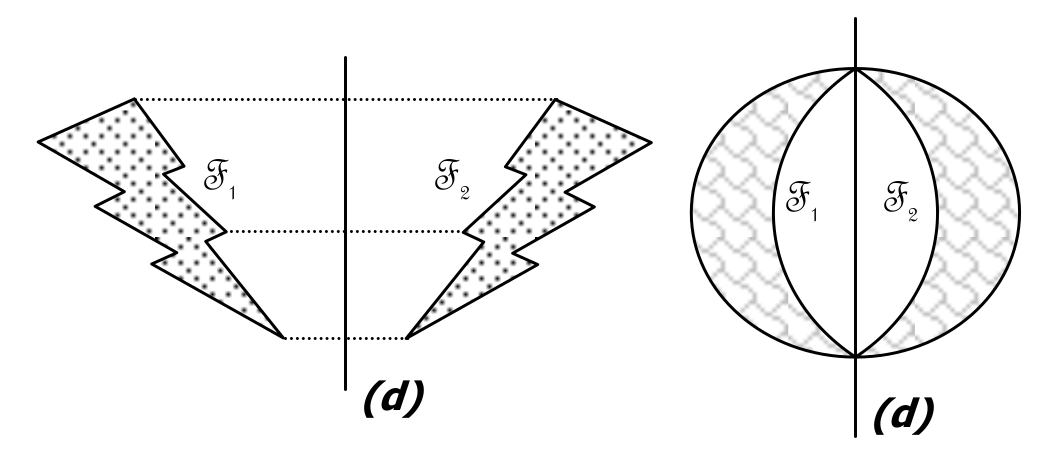
\includegraphics[scale=0.35]{def}
		\end{center}
	
		\iftoggle{eleve}{%
			\vspace*{0.2cm}
			\hrulefill
			
			\vspace*{0.2cm}
			\hrulefill
		}{%
			La figure $F_2$ est la symétrique de $F_1$ par rapport à la droite $(d)$.
		}
		
	\end{myexs}

\newpage

\section{Médiatrice}


\begin{mydef}
	La médiatrice d'un segment est la droite \kw{perpendiculaire à ce segment} et qui \kw{passe par son milieu}.
\end{mydef}


\begin{myex}
	La droite $(d)$ est la médiatrice du segment $[AB]$.
	
	\begin{center}
		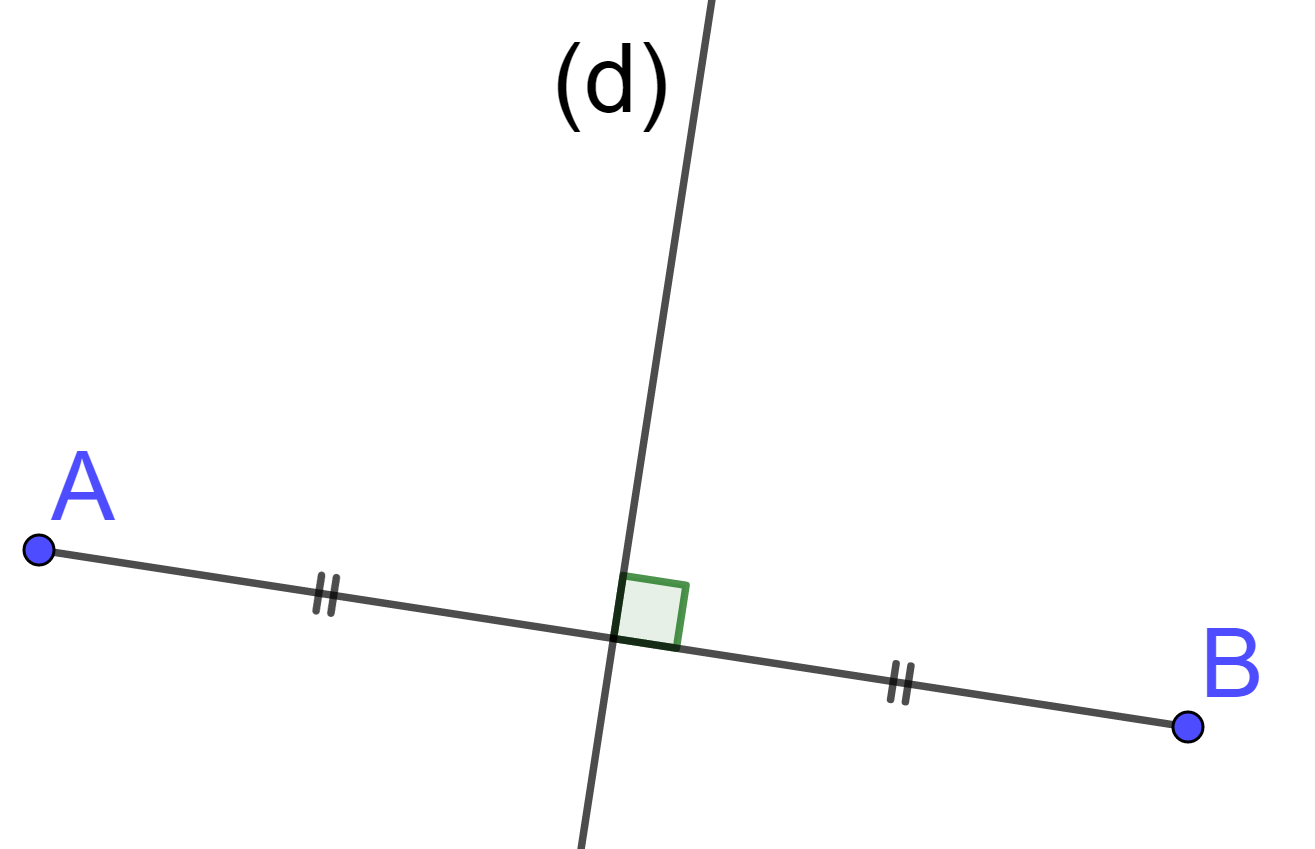
\includegraphics[scale=0.15]{med1}
	\end{center}
\end{myex}

\begin{myprops}
	\begin{itemize}
		\item \textbf{Si} un point appartient à la médiatrice d'un segment, \textbf{alors} ce point est à la même distance des extrémités de ce segment.
		\item \textbf{Si} un point est à la même distance des extrémités d'un segment, \textbf{alors} il appartient à la médiatrice de ce segment.
	\end{itemize}
\end{myprops}


\begin{myexs}
	\begin{multicols}{2}
		
		\begin{enumerate}
			
			
			\item  Le point $D$ appartient à la médiatrice $(d)$ du segment $[AB]$, donc $AD=BD$.
			
			\vspace*{0.5cm}
			\begin{center}
				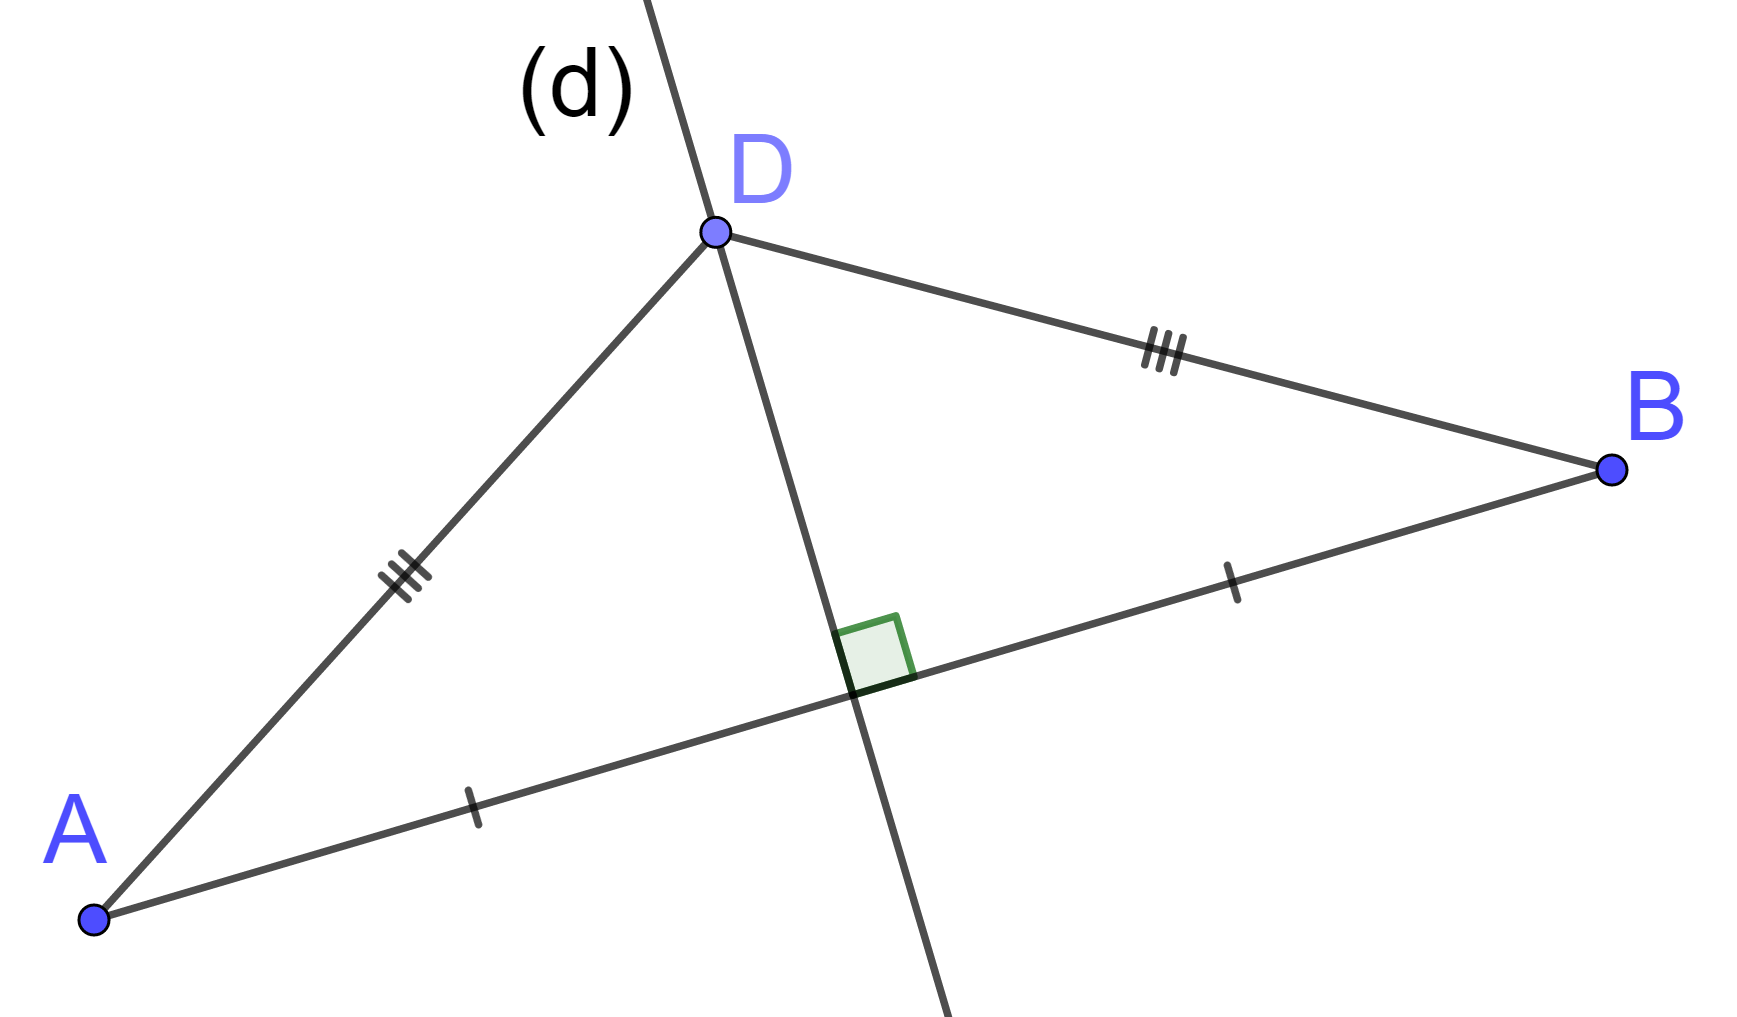
\includegraphics[scale=0.15]{med2}
			\end{center}
			
			
			\item On a $EG=GF$, $EH=HF$ et $EI=IF$, donc les points $G$, $H$ et $I$ appartiennent tous à la médiatrice du segment $[EF]$.
			
			\begin{center}
				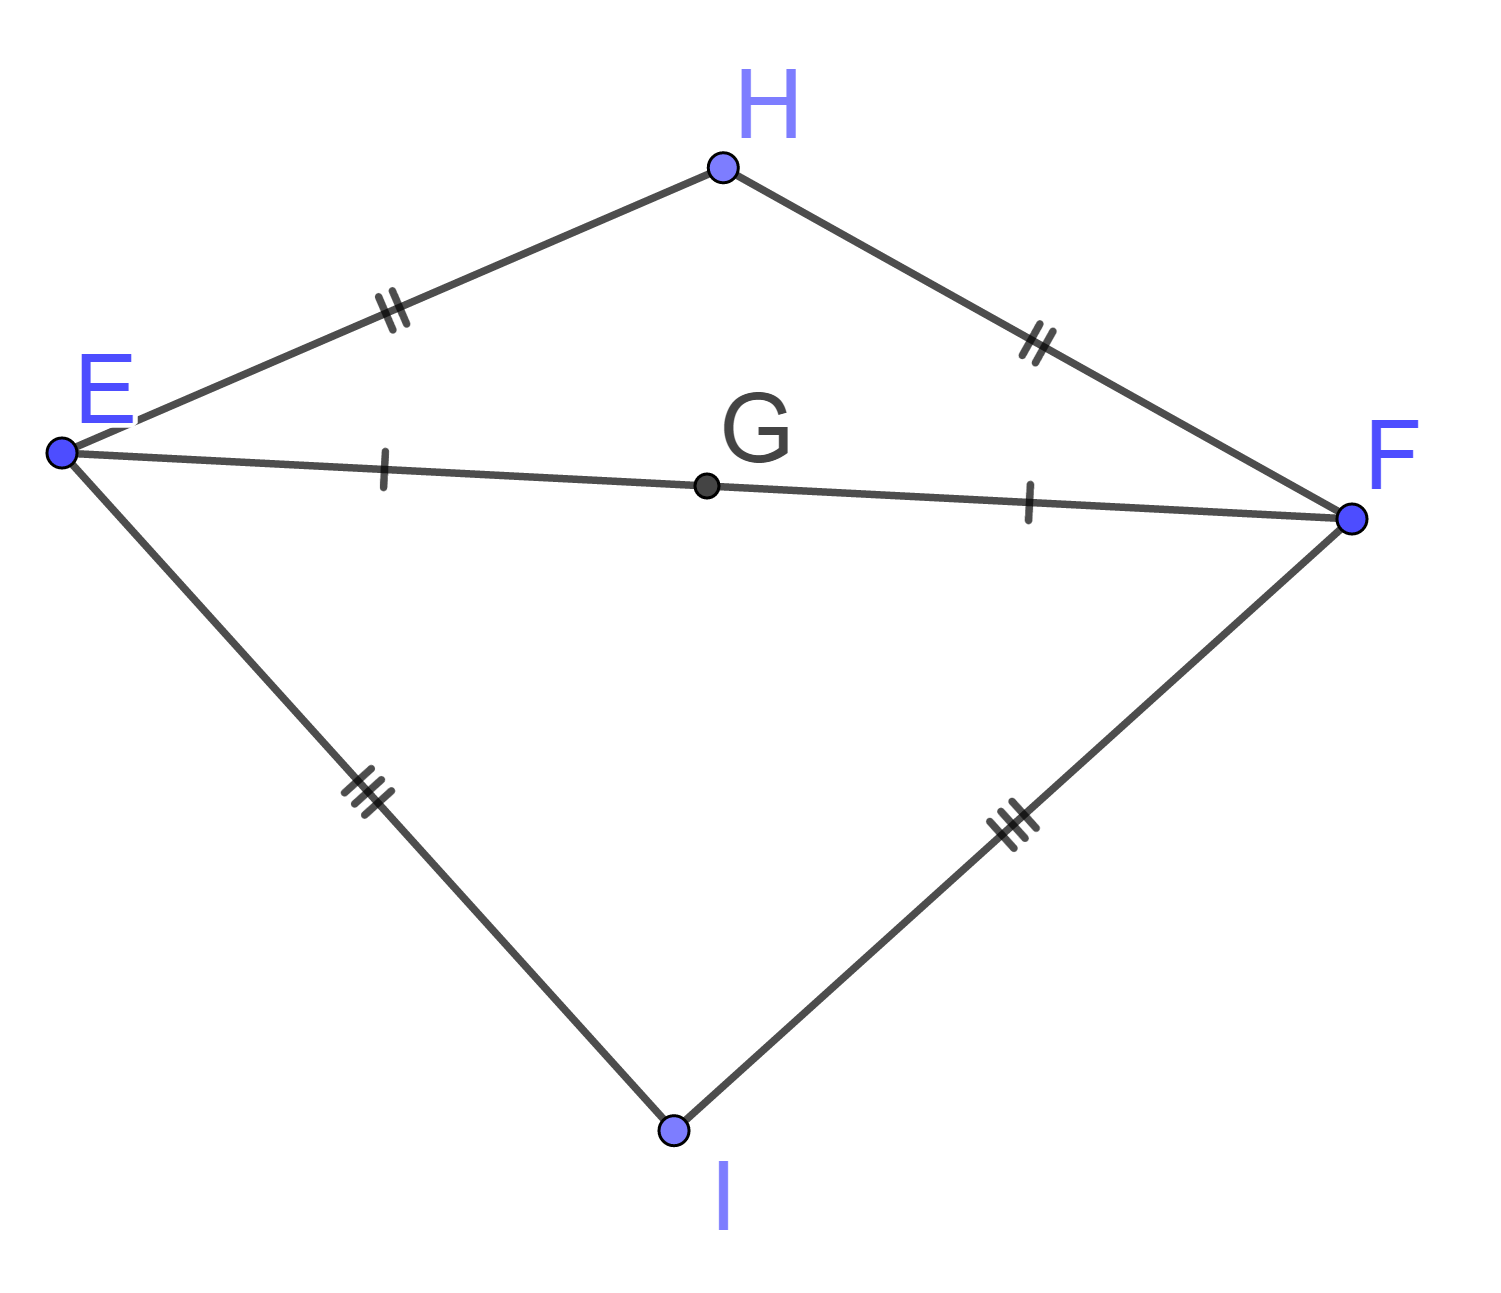
\includegraphics[scale=0.13]{med3}
			\end{center}
			
		\end{enumerate}
	\end{multicols}
	
	
	
\end{myexs}

\begin{mymeth}
	Pour tracer la médiatrice d'un segment $[AB]$ au compas et à la règle non graduée :
	
	\begin{enumerate}
		\item choisir un écartement plus grand que la moitié du segment;
		\item placer la pointe du compas en $A$ et tracer un arc de cercle;\label{step1}
		\item en gardent le même écartement, placer la pointe du compas en $B$;
		\item tracer un arc de cercle qui coupe le premier;
		\item placer le point $I$ à l'intersection;\label{step2}
		\item refaire les étapes \ref{step1} à \ref{step2} avec un autre écartement en nommant le point $J$;
		\item tracer la droite $(IJ)$ médiatrice du segment $[AB]$.
		
	\end{enumerate}
\end{mymeth}


\section{Propriétés de la symétrie}

\begin{myprop}
	\kw{Si} deux droites sont perpendiculaires à une même troisième droite, \kw{alors} ces deux droites sont parallèles.
\end{myprop}


\begin{myex}
	\begin{multicols}{2}
		\kw{On sait que} $(d_1)$ et $(d_2)$ sont toutes deux perpendiculaires à $(D)$.\\
		\kw{Donc} $(d_1)$ et $(d_2)$ sont parallèles.
		
		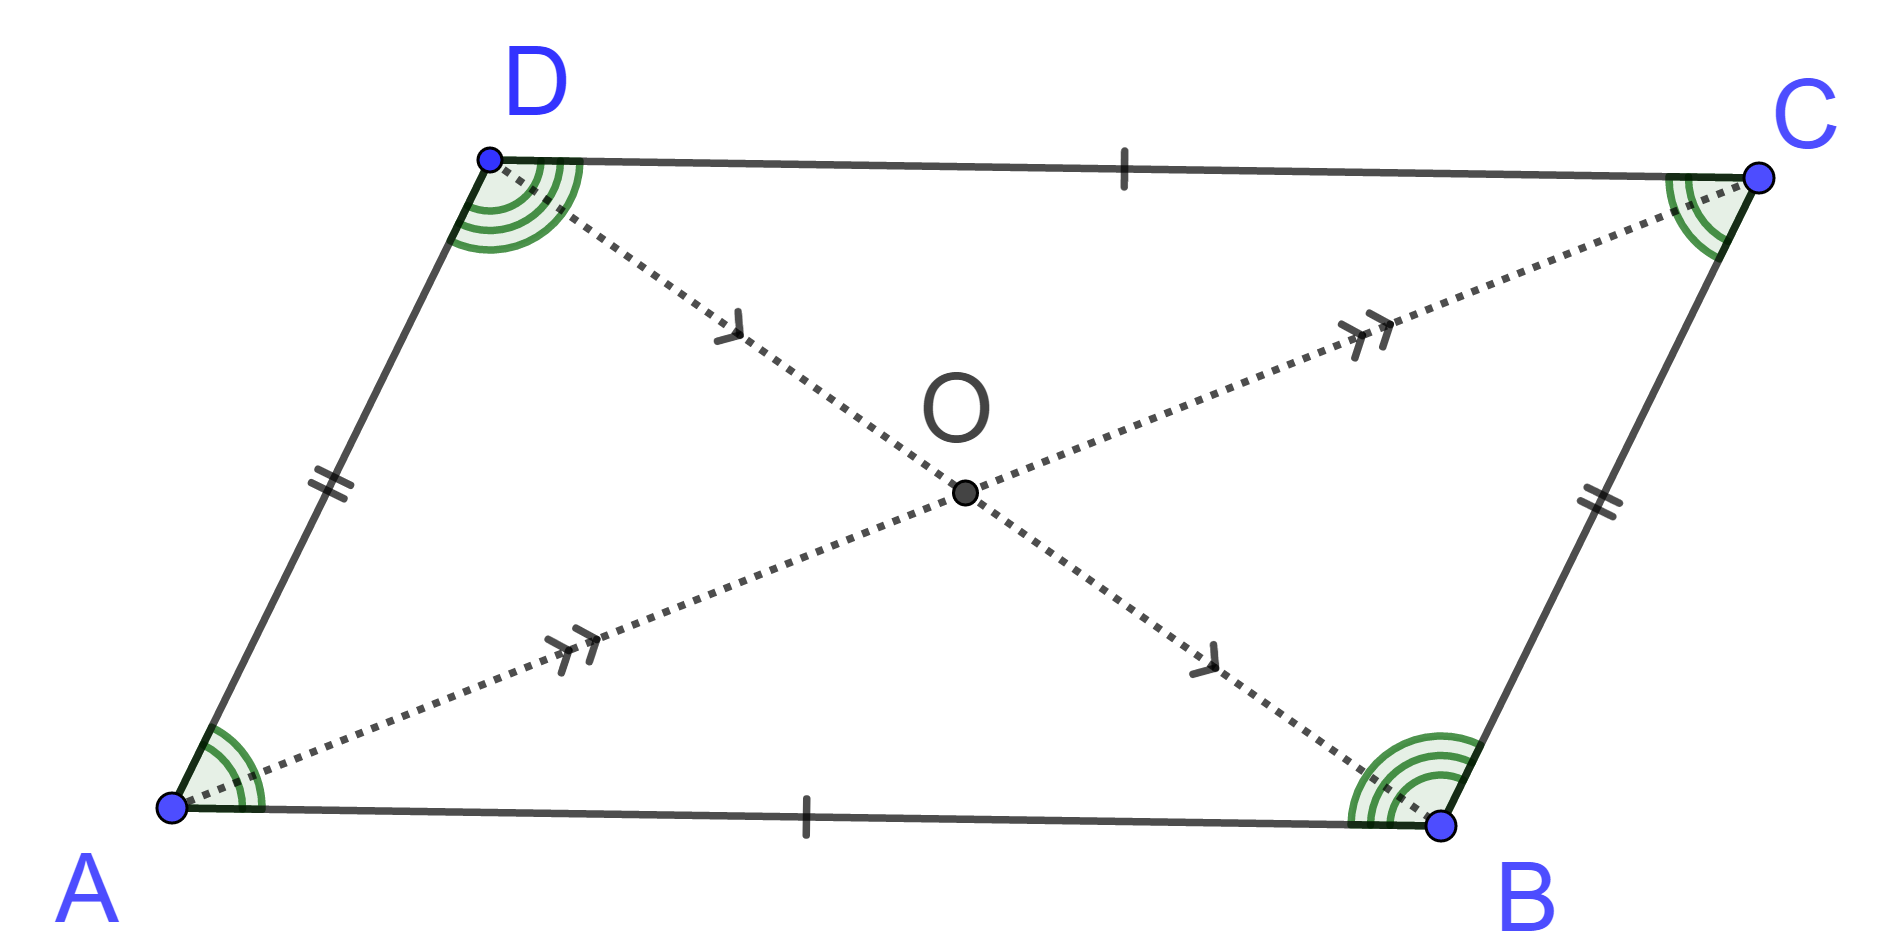
\includegraphics[scale=0.6]{img/para2}
	\end{multicols}
	
\end{myex}


\begin{myprop}
	\kw{Si} deux droites sont parallèles, \kw{alors} toute perpendiculaire à l’une est perpendiculaire à l’autre
\end{myprop}


\begin{myex}
	\begin{multicols}{2}
		\kw{On sait que} $(d_1)$ // $(d_2)$ et $(d_1) \perp (D)$\\
		\kw{Donc} $(d_2) \perp (D)$.
		
		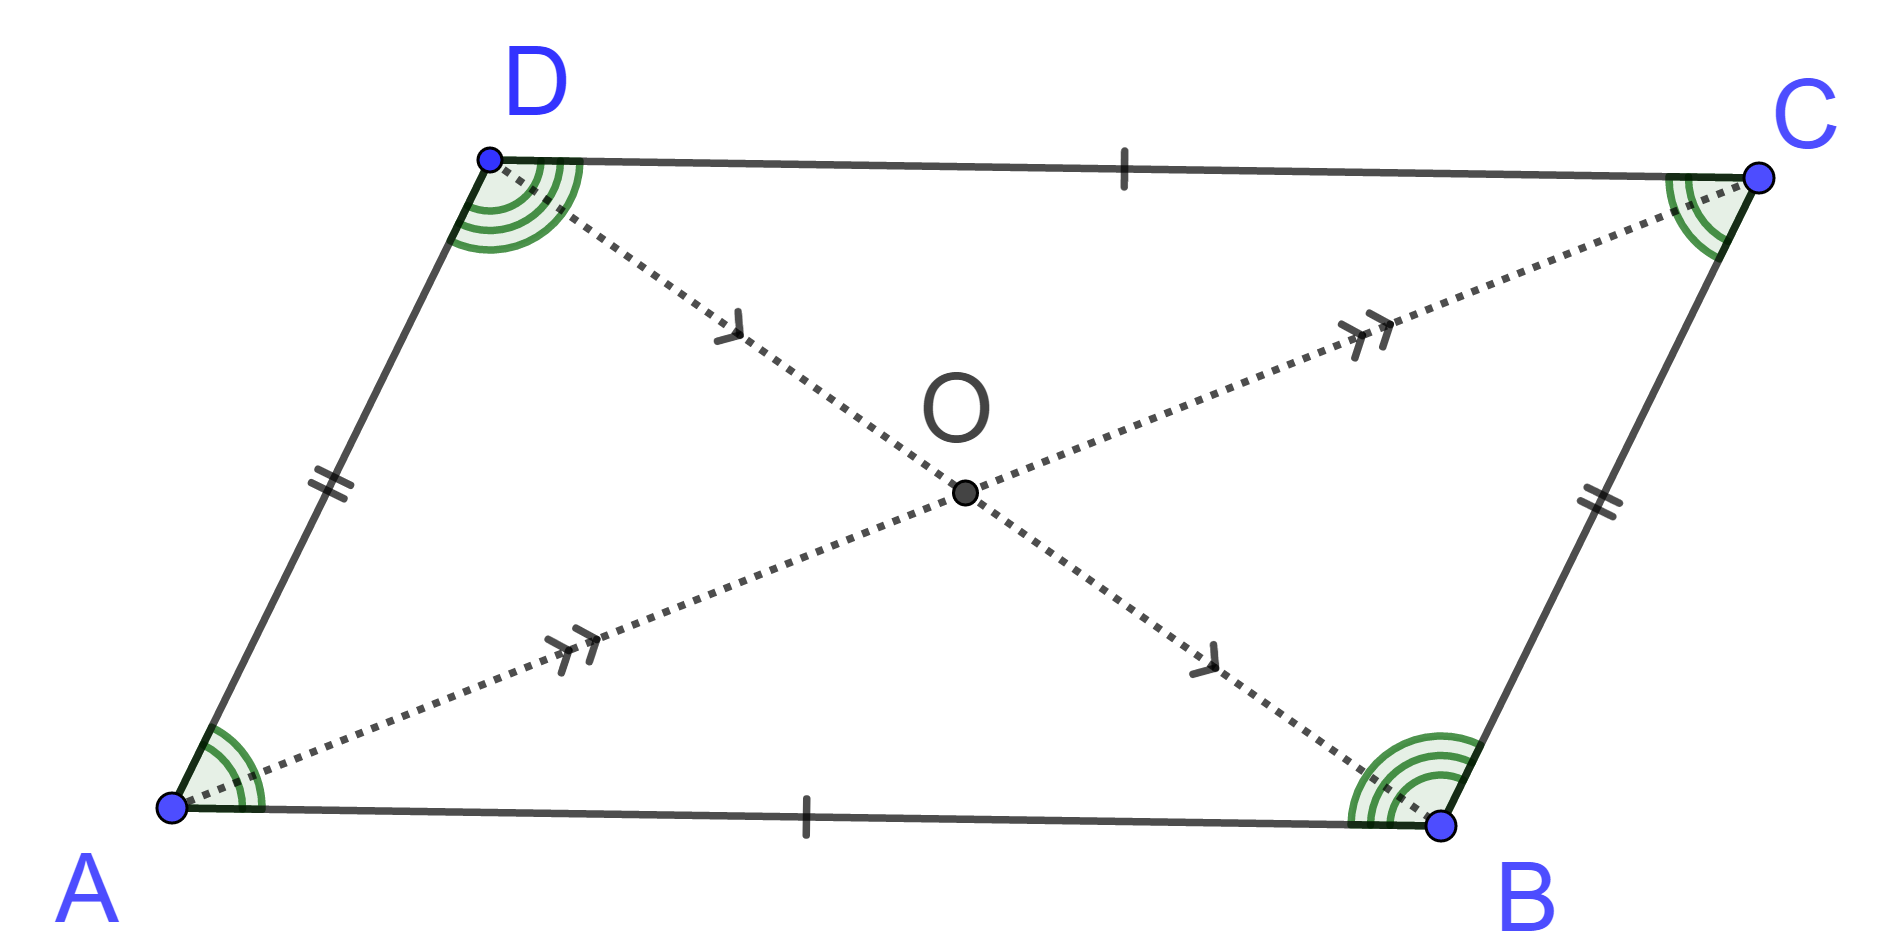
\includegraphics[scale=0.6]{img/para2}
	\end{multicols}
	
\end{myex}

\begin{myprop}
	\kw{Si} deux droites sont parallèles à une même troisième, \kw{alors} ces deux droites sont parallèles entre elles.
\end{myprop}

\begin{myex}
	\begin{multicols}{2}
		\kw{On sait que} $(d_1)$ // $(d)$ et $(d_2) // (d)$\\
		\kw{Donc} $(d_1) \perp (d_2)$.
		
		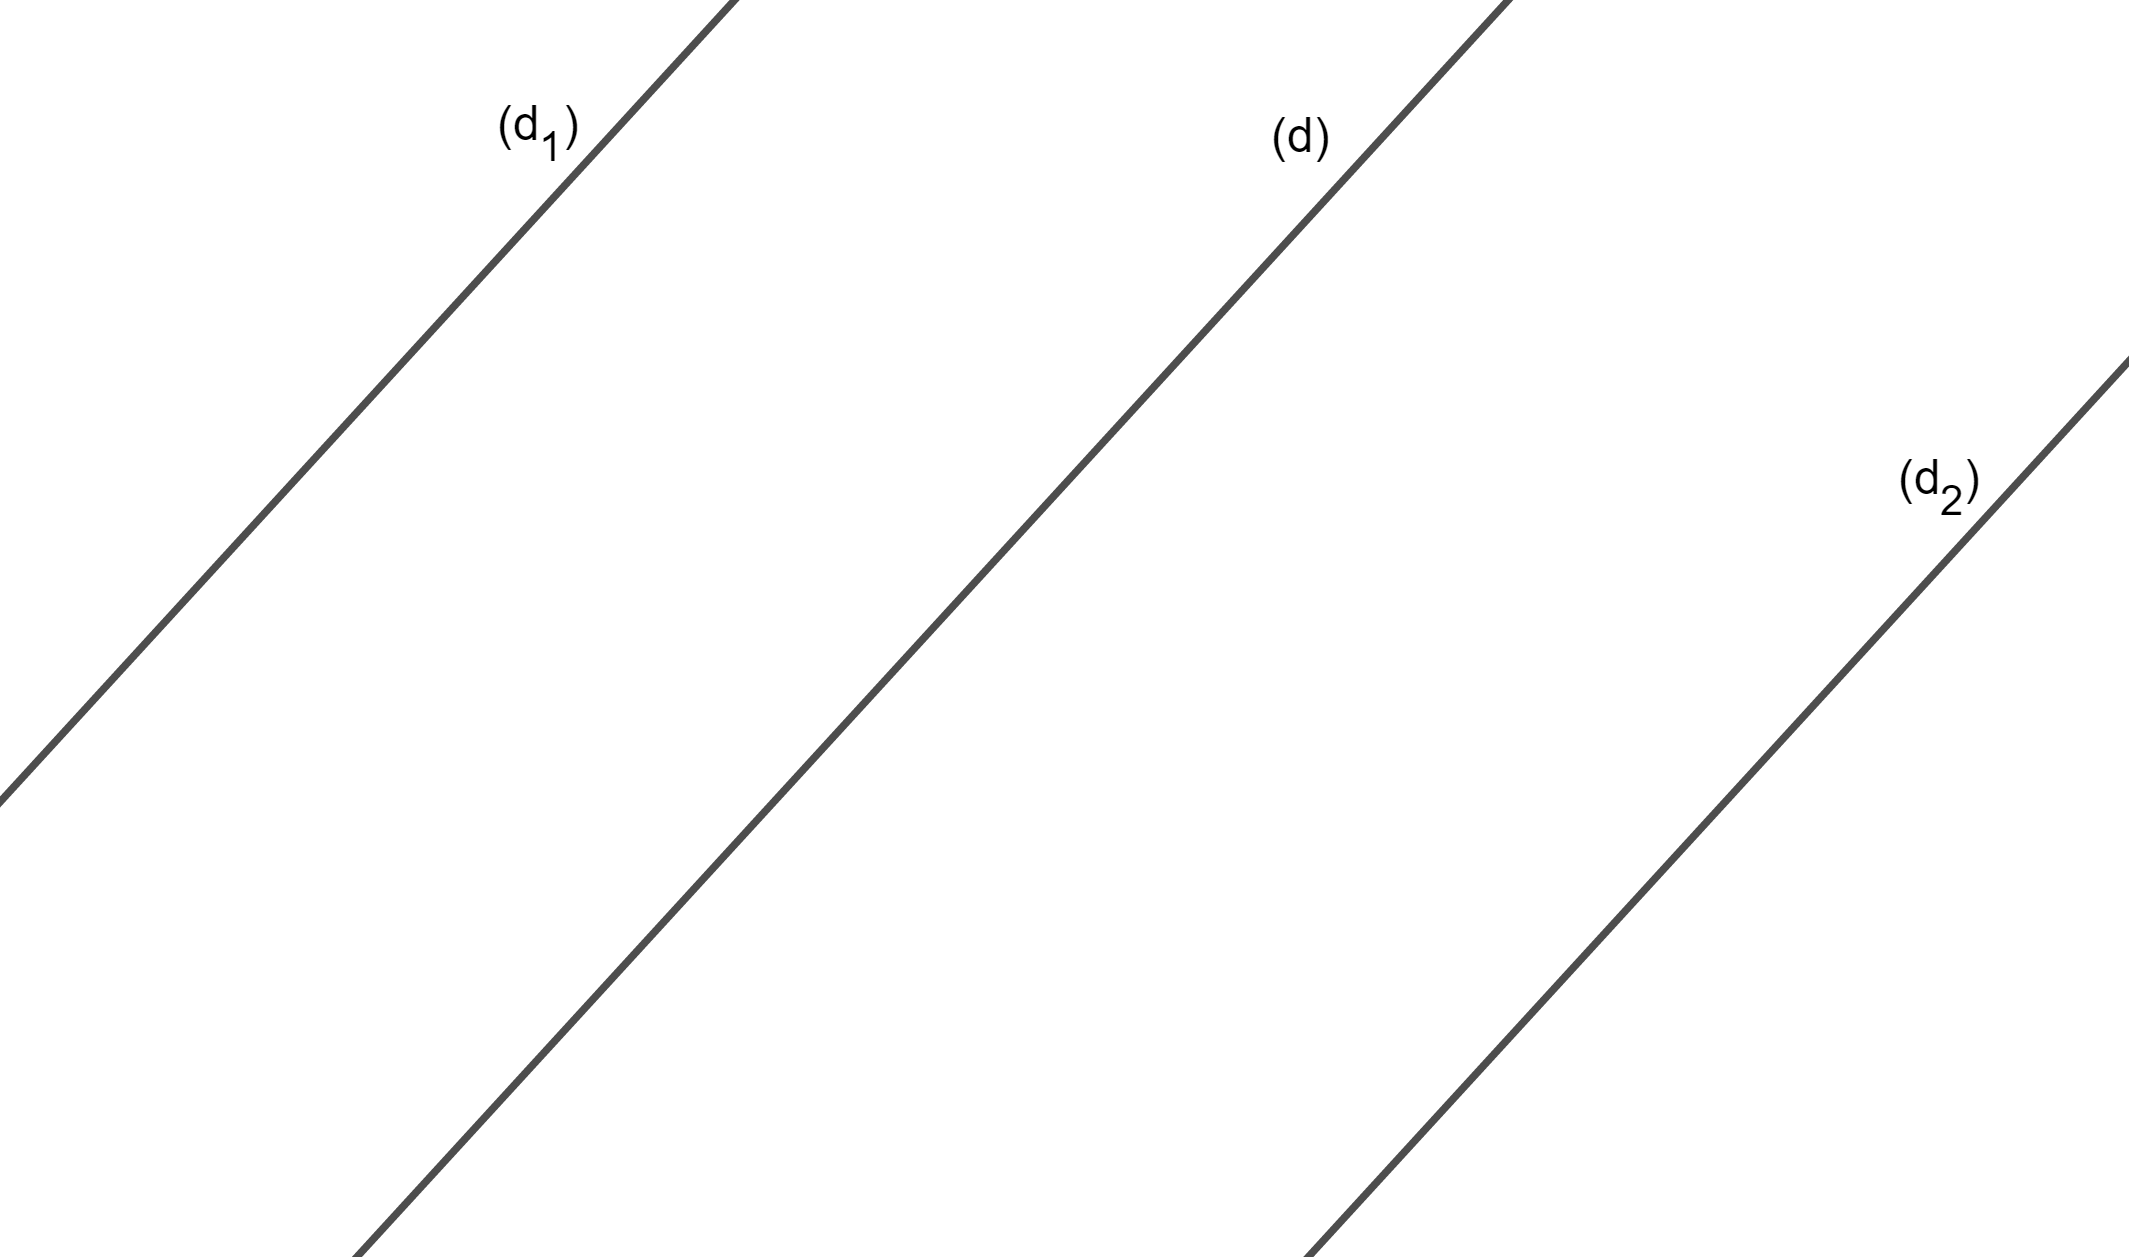
\includegraphics[scale=0.1]{img/para3}
	\end{multicols}
	
\end{myex}



\end{document}